Calcula el volumen del sólido acotado por la superficie \( z=\sin y \), los
planos \( x=1 \), \( x=0 \), \( y=0 \) \( y= \frac{\pi}{2} \), y el plano \( xy \).
\begin{solution}
    La gráfica de este sólido luce más o menos como
    \begin{figure}[H]
        \begin{center}
            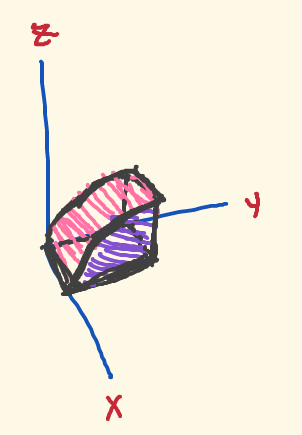
\includegraphics[width=0.3\textwidth]{img/Ej3/ej10.png}
        \end{center}
    \end{figure}
    Este volumen se puede calcular con el principio de Cavalieri con las secciones transversales
    \[
        C_x=\set{(x,y,z):0 \leq y\leq \frac{\pi}{2},0\leq z\leq \sin y},
    \]
    donde $0\leq x\leq 1$. Es decir, las intersecciones entre el sólido y los planos paralelos al 
    plano \( yz \).
    Por lo tanto el volumen de esta figura es 
    \begin{align*}
        \int_0^1
        \int_0^{\frac{\pi}{2}}
        \sin y
        \,dy
        \,dx
        &=
        \int_0^1
        -\cos \left( \frac{\pi}{2} \right)+
        \cos(0)
        \,dx\\
        &=
        \int_0^1 1 \, dx
        \\
        &=
        1
    \end{align*}
\end{solution}
